\documentclass[a4paper, 10pt]{article}
    \usepackage[utf8]{inputenc}
    \usepackage{fullpage}
    \usepackage{enumitem}
    \usepackage{graphicx}
    \graphicspath{{images/}}
    \usepackage[urlcolor=blue]{hyperref}

    % No indent on new paragraph
    \setlength{\parindent}{0em}

    \setlength{\parskip}{1em}
    \renewcommand{\baselinestretch}{1.15}

    \title{COP 5615 - Project 2 Bonus Report}
    \author{Vaibhav Yenamandra ($1931$-$4050$)\\ email: \href{vyenaman@ufl.edu}{vyenaman@ufl.edu} }
    \date{\today}

    \begin{document}

    \begin{center}
      \textbf{COP5615 - Project 2 Bonus Report}
    \end{center}
    \textbf{Author:} Vaibhav Yenamandra ($1931$-$4050$)\\
    \textbf{Date:} \today
    % \maketitle

    \section{Gossip Robustness to Message Loss}
    \begin{figure}[h]
      \caption{$\log ($Gossip Convergence Time$)$ v/s Message Failure Probability}
      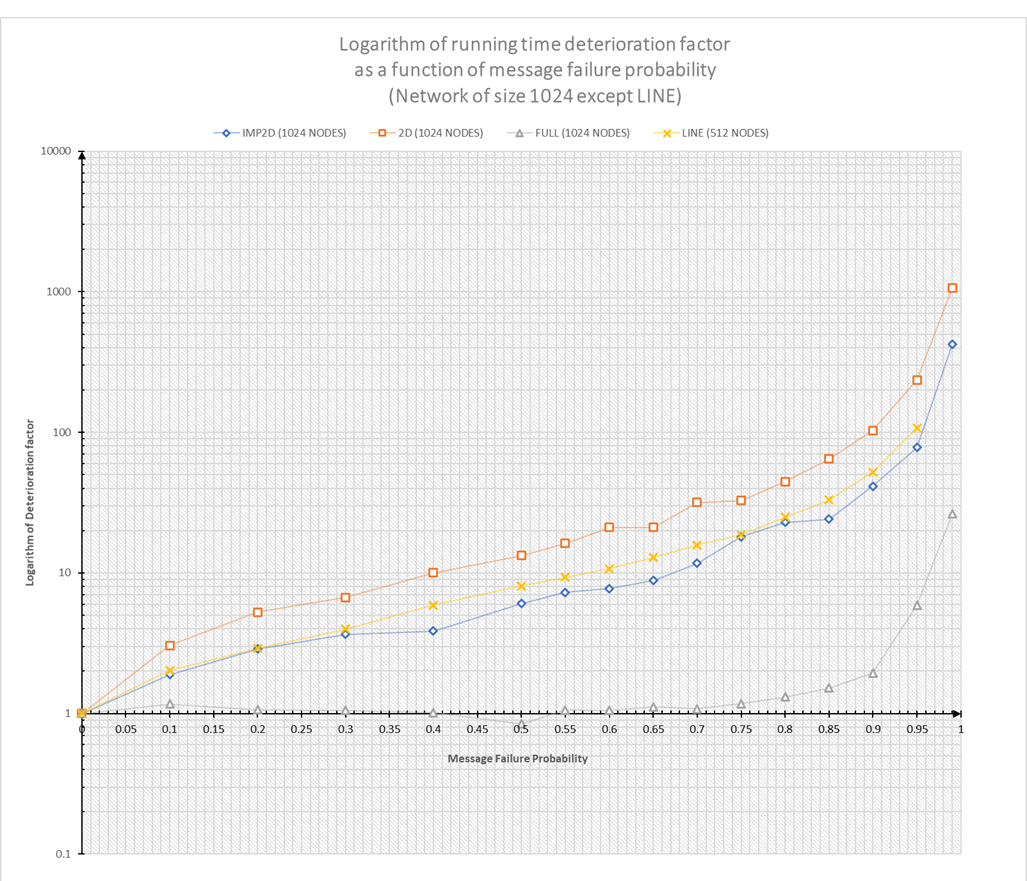
\includegraphics[width=\textwidth]{project2_bonus}
      \label{fig:slowdown}
    \end{figure}

    In this part of the report I test a fixed size network that randomly loses messages between nodes in order to see which topologies are robust to these kinds of lossy networks.

    For testing fault tolerance of the Gossip protocol, I added an attribute to each node in the network called ``failure probability''. It parametrizes the likelihood of an message being discarded by a node, this is done so as model networks where the nodes are communicating via protocols such as UDP in a network where packets are randomly dropped.

  Figure 1 plots the logarithm of convergence time for various topologies of size 1024 vs the message failure probability. Each of curves is scaled to represent the slowdown factor defined as the ratio of convergence time with failure, to convergence time without failure, all of the curves start at 1 and move upwards hence.

    Some points to note:

    \begin{enumerate}
      \item{Fully connected networks turn out to be the most robust of all. They are not affected till failure probability is as high as $90\%$}
      \item{The slowdown factor ($f$) is highly correlated with the inverse of the failure probabilty ($p$), with $99\%$ spearman regression coefficients for each of the following equations:}

      \begin{equation}
        f_{imp2d}(p) = -2.332 + \frac{4.2293}{1-p}
      \end{equation}
      \begin{equation}
        f_{2d}(p) = -6.1826 + \frac{10.7223}{1-p}
      \end{equation}
      \begin{equation}
        f_{full}(p) = 0.3721 + \frac{0.2580}{1-p}
      \end{equation}
      \begin{equation}
        f_{line}(p) = -3.5215 + \frac{5.5613}{1-p}
      \end{equation}

      \item{The factor $f$ can be multiplied in to get the actual running convergence time in the presence of failure probability.}
    \end{enumerate}

    \begin{figure}[h]
      \caption{Susceptibility to failure v/s Message Failure Probability}
      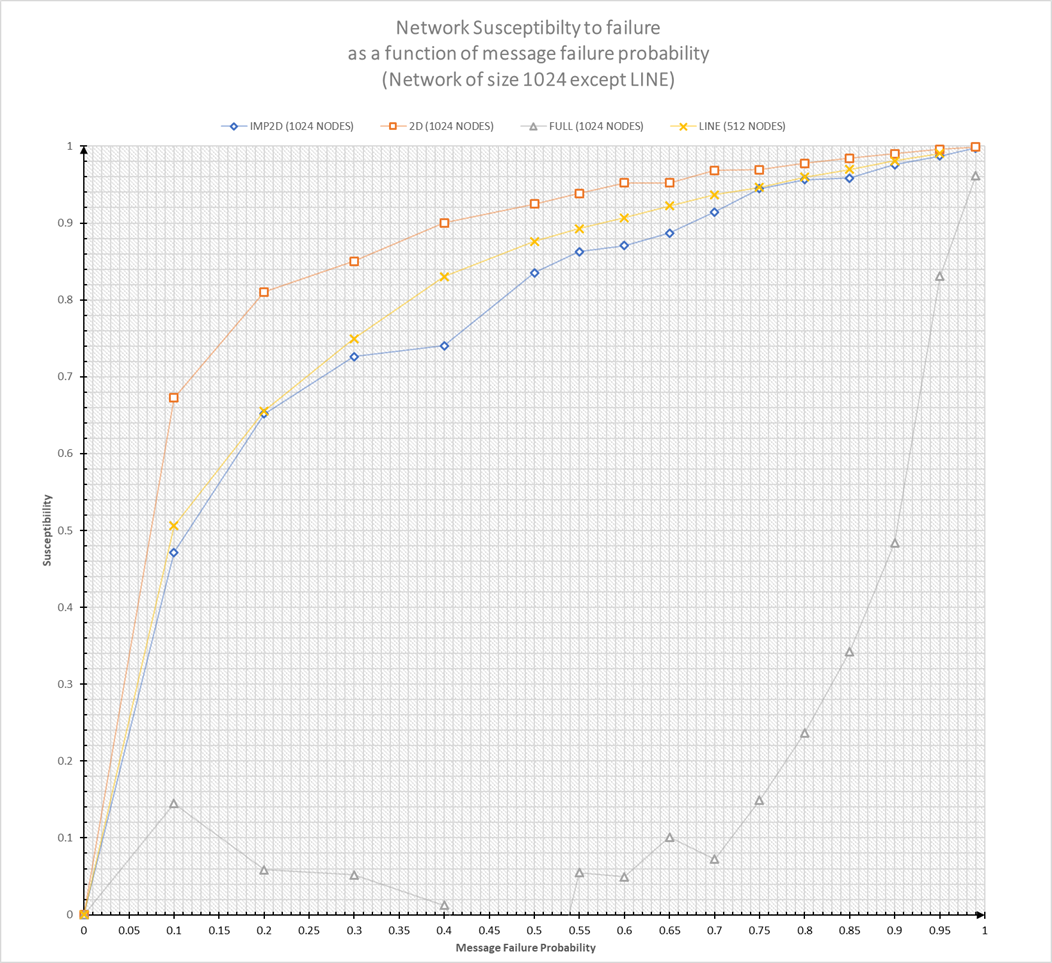
\includegraphics[width=\textwidth]{project2_bonus_susceptibility}
      \label{fig:susceptibility}
    \end{figure}

    A topology's robustness is better illustrated by defining the susceptibility ($S$) of a network to failure as $S_{topology} = 1 - 1/f_{topology}$, this is plotted in Figure ~\ref{fig:susceptibility}. It is evident that as far as robustness is concerned, the order is: full $>$ Imperfect 2D $>$ 2D.

    We can adjust the convergence times in the presence of failure as follows:

    $t_{failure, topology} = t_{regular, toplogy} \cdot f_{topology}(p_{failure})$
\end{document}
